%------------------------------------------------------------------------------------------------------------------------------------------
%  Teorie
%------------------------------------------------------------------------------------------------------------------------------------------
\chapter{TEORETICKÁ VÝCHODISKA}
\par Pro plné pochopení, výběru a případném vypracování platformz je potřeba si objasnit a vysvětlit několik témat. Jsou to především \textit{Vývojové platformy low-code}, výsledná platforma by měla splňovat tuto definici. Dále si objasníme pojemy \textit{Bussiness intelligence} (platforma bude z části pracovat s touto oblastí) a \textit{Platforma pro pokročilou vizualizaci dat} -- pro snadné používání uživatelského rozhraní. A vzhledem k tomu že výsledná platforma musí do určité části pracovat s uživatelskými právy a spravovat uživatele, objasníme si pojem \textit{Server pro řízení přístupu a identity}

\section{Vývojové platformy low-code}
\par Vývojové platformy low-code jsou celkem nový pojem, tyto produkty začali vznikat, protože malé a střední podniky potřebovali vytvořit rychle a za použití menšího počtu vývojářů aplikace, které mohou být nadále rychle spravovány. \ref{pcmag-no-coding}

\par Toto v podstatě znamená, že vývojáři mohou rychle měnit software na základě uživatelských požadavků, což má za následek spokojenější uživatele, uživatelsky přívětivější software a toto všechno za minimálního použití ručního programování. Takovéto platformy neeliminují programování jako takové, ale napomáhají rychlejšímu vývoji, tak že poskytují vizuální nástroje a napomáhají konfiguraci datových modulů a pomáhají eliminovat problémy spojené s  datovou integrací. - http://www.cio.com/article/2845378/development-tools/use-low-code-platforms-to-develop-the-apps-customers-want.html

\paragraph{Výhody low-code platforem}
\begin{itemize}
  \item \textbf{Produktivita:} Systémy mohou být vyvýjeny a nasazeny během menšího časového rozmezí, oproti klasickému programování.
  \item \textbf{Reakční schopnost:} Vývojář může často zvolit různé druhy platforem na kterých bude výsledný produkt fungvat, od mobilních aplikací, až po webové služby.
  \item \textbf{Spolehlivost:} Aplikace mohou být aktualizovány mnohem rychleji, což má za následek jejich stabilitu a spolehlivost.
  \item \textbf{Úspora času a peněz:} Vývojáři mohou vytvořit mnohem více funkcionality za kratší čas, z čehož plyne že si firma může dovolit mensí počet programátorů.
  \item \textbf{Zaměření na samotný vývoj:} Zaměřením na to co má aplikace dělat, a ne jak to má dělat, programátoři se mohou zaměřit na funkcionalitu a uživatelskou spokojenost. Při vývoji je možné se zaměřit také více na uživatelské požadavky mnohem rychleji.
\end{itemize}
http://sdtimes.com/low-code-development-seeks-accelerate-software-delivery/

\subsection{Příklady low-code platforem}
\paragraph{Microsoft PowerApps} Vývojová platforma od firmy Microsoft, která dovoluje vytvořit během několika málo kliknutí aplikaci pro mobilní platformy a také jako webové služby. Při spojením této platformy a aplikace Power BI vzniká velice robustní vývojářský nástroj, díky kterému je možné rychle integrovat produkční data do aplikace, kterou budou uživatelé rádi používat.
\paragraph{Zoho Creator} Výhodou této platformy je využití techniky \uv{\tt{drag-and-drop}}, která umožňuje vytvářet aplikace a převážně jejich uživatelské rozhraní bez nutnosti psát jakýkoliv kód. https://reviews.financesonline.com/p/zoho-creator/
\paragraph{Rollbase} Při používání této platformy vývojář jako první definuje objekty, jejich vlastnosti a vztahy mezi těmito objekty. Po překonání tohoto kroku máme již plně funkční webovou aplikaci, která je funkční napříč všemi mobilními zařízeními. https://www.progress.com/blogs/what-is-a-low-code-platform
\paragraph{Openshift} Platforma pro vývoj webovým a mobilních aplikací, postavená na kontejnerech, které zajišťuí rychlý vývoj a možnost dedikovat vývojáře na vytvoření jednoduchých funcionalit jako samostatné aplikace \footnote{Takovýmto aplikacím se říka Microservice https://smartbear.com/learn/api-design/what-are-microservices/}, které za pomocí Openshiftu vytvoří velkou a komplexní aplikaci.
\begin{figure}[h]
\centering
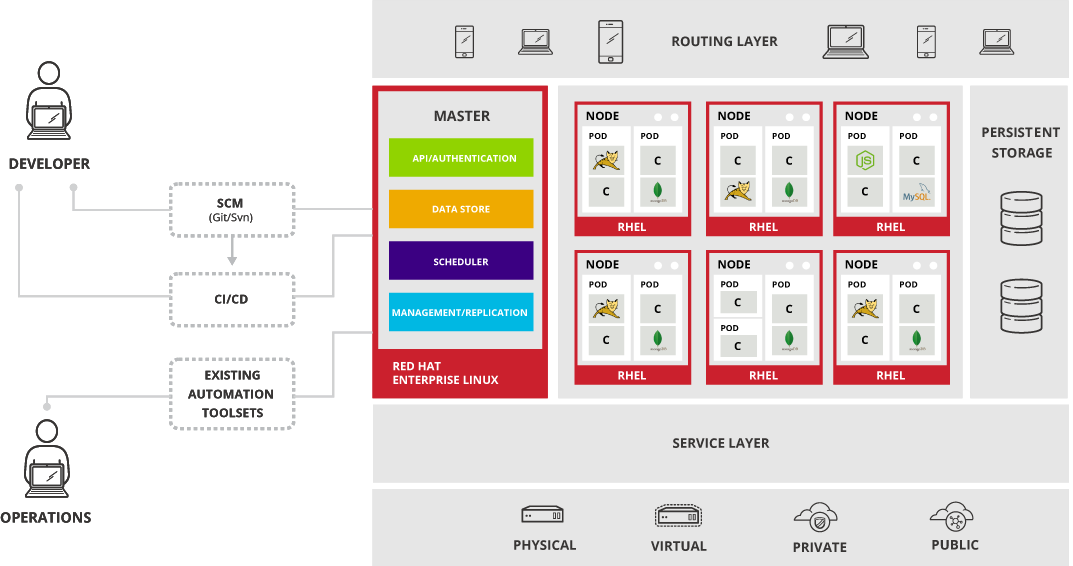
\includegraphics[width=\textwidth]{openshift}
\caption{Znozornění jednotlivých vrstev v platformě openshift.}
\end{figure}

\subsection{Platforma jako služba -- Paas}

\section{Bussiness Intelligence}

\subsection{Big data}

\subsection{Datamining}

\subsection{Extraction, Transaction, Loading}

\subsection{NoSql databáze}
\cite{nosql}

\section{Platforma pro pokročilou vizualizaci dat}
\subsection{Single page aplikace}
\subsection{Dynamická a interaktivní vizualizace dat}
\subsection{Webová služba RESTful}
Restufl web APIs

\section{Server pro řízení přístupu a identity}
\url{http://www.sersc.org/journals/IJMUE/vol9_no9_2014/9.pdf}

\subsection{JSON Web Token}
https://tools.ietf.org/html/rfc7519
https://scotch.io/tutorials/the-anatomy-of-a-json-web-token
